% !TEX root = ../main.tex

\chapter{实现与评估} \label{ch:implement}

\section{编译链及定理证明的实现}

如第~\ref{sec:overview}节中所述,我们主要使用了交互式定理证明器Coq实现
程序语言定义及编译算法,并完成相关定理的形式化证明。
Coq主要是用OCaml语言实现的,它支持数学断言的表示,并且能够检查这些断言的证明,
从其形式化的构造证明中提取出验证程序~\cite{paulin2011introduction}。
作为一种编程语言,Coq是一种依赖类型的函数式编程语言;作为一种逻辑系统,它实现了一种高阶类型理论。
其中,编译链的PCF语法分析器(Parser)部分在OCaml中实现,它分析PCF程序文本并
在顶层Coq模块中添加需要进行编译的PCF源程序。之后的编译过程及验证在Coq中实现,
并链接到Coq中的Vellvm抽象语法树。

\subsection{PCF语法分析器}
我们没有直接去编写实现词法解析和语法解析功能的OCaml代码,而是
使用ocamllex和ocamlyacc~\cite{smith2007ocamllex}作为词法和语法解析器的生成器。
该PCF语法分析器的结构如图~\ref{fig:parser}所示。

Ocamllex可以从附加了语义行为的正则表达式(Regular Expression)集合中生成词法分析器。
我们首先在\textit{lexer.mll}中定义了直接风格PCF语言的词法解析规则,
包括输入文本中各种词法单元的模式匹配和对应的操作,然后使用ocamllex
生成词法分析器的OCaml代码\textit{lexer.ml}。
在\textit{lexer.ml}文件中,词法分析函数将词法分析缓冲区(Lexer Buffer)作为参数,
生成标记流(Tokens)。
词法分析缓冲区是在OCaml标准库模块Lexing中实现的抽象数据类型,它维护分析函数当前的状态,
并可以从输入获取内容对缓冲区进行填充~\cite{leroy2021ocaml}。
分析函数会将缓冲区中的字符与词法规则中定义的正则表达式进行匹配,直到输入的前缀符合某条规则,
执行相应的操作。如果符合多条规则,就按照最长匹配原则。
Ocamlyacc会根据语法规则\textit{grammar.mly}生成语法分析器的接口\textit{grammar.mli}
和实现\textit{grammar.ml}。语法解析函数的参数包括上文中提到的词法分析器和词法分析缓冲区。
它将词法分析得到的标记流解析为抽象语法树。之后,我们使用\textit{printer.ml}读入PCF程序
在OCaml中的抽象语法树打印出它的Coq程序并将其写入Coq编译链的顶层模块,这样就可以直接在Coq中使用它了。

\begin{figure}[htbp]
    \centering
    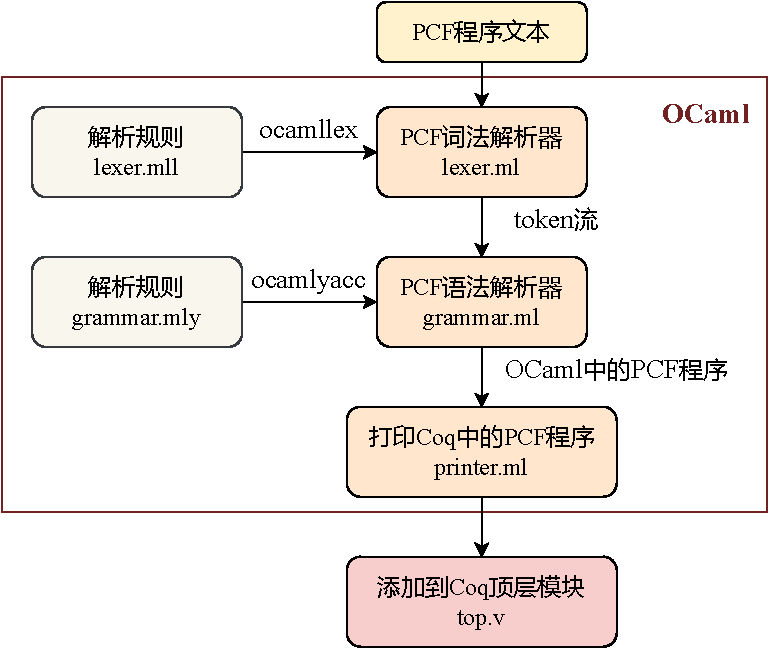
\includegraphics[width=0.8\linewidth]{figures/pcfparser.pdf}
    \caption{PCF语法分析器结构}\label{fig:parser}
\end{figure}

\subsection{编译算法实现}

我们在Coq中完成了PCF、CPS和SSA程序语言的定义以及从PCF源程序到Vellvm抽象语法树的编译链。
如上一节所述,我们已经使用PCF语法分析器在Coq顶层编译模块得到了PCF程序的抽象语法树。
除了

PCF程序到SSA程序的两步转换算法及正确性验证均在Coq中实现,位于文件夹FrontEnd目录下。
由SSA程序生成LLVM IR代码的过程也在Coq中进行实现,因为经验证的LLVM,即Vellvm也是在Coq中实现。
将Coq中的SSA程序直接编译到Vellvm中的抽象语法树,即可生成LLVM IR程序。

在编译算法正确性证明过程中使用的小步操作语义是关系型的,即两个程序状态之间的关系。
这样的设计对于证明来说很方便,但是无法直接运行程序得到结果。
为了对操作语义和转换算法进行初步测试,使用Coq为三种语言分别构建解释器(Interpreter),
从而能够执行相应的程序,得到程序返回的结果。其中,发散的定义要取决于对最大步数的限定,即解释器的fuel。
解释器每走一步都会消耗一个fuel,如果fuel消耗完程序还没有终止或出错,就可以认为程序发散了,返回超时状态(Timeout)。
进行解释器测试主要是为了找出操作语义和转换算法中的问题,为接下来的证明减少阻碍。形式化验证过程本身与解释器没有关系。

\subsection{定理证明的实现}

\section{各部分Coq代码评估}

各主要模块类别和内容的代码行数(Lines of Code, LOC)如下表~\ref{tabeval}。可以看到,相关定理的证明即转换算法验证部分是工作量占比最大的。

\begin{table}
    \linespread{1.25}
    \small
    \centering
    % \vspace{-20pt}
    \caption{Coq代码LOC评估}\label{tabeval}
    \begin{center}
    \begin{tabular}{|l|l|l|l|}
    \hline
    代码类别 & 代码实现内容 & LOC & 行数占比(\%) \\
    \hline
    \multirow{3}{*}{程序语言定义} & PCF & 171 & \multirow{3}{*}{23.9} \\
        & CPS & 228 & \\
        & SSA & 303 & \\
        \hline
    \multirow{3}{*}{转换算法} & PCF$\rightarrow$CPS & 148 & \multirow{3}{*}{24.5} \\
        & CPS$\rightarrow$SSA & 251 & \\
        & SSA$\rightarrow$LLVM IR & 318 & \\
        \hline
    \multirow{4}{*}{形式化验证} & PCF$\rightarrow$CPS前向模拟 & 364 & \multirow{4}{*}{51.6} \\
        & CPS$\rightarrow$SSA前向模拟 & 696 & \\
        & 前向模拟组合 & 49 & \\
        & 后向模拟 & 404 & \\
        \hline
    \end{tabular}
    \end{center}
\end{table}

